\documentclass[tikz,border=5pt]{standalone}
\begin{document}
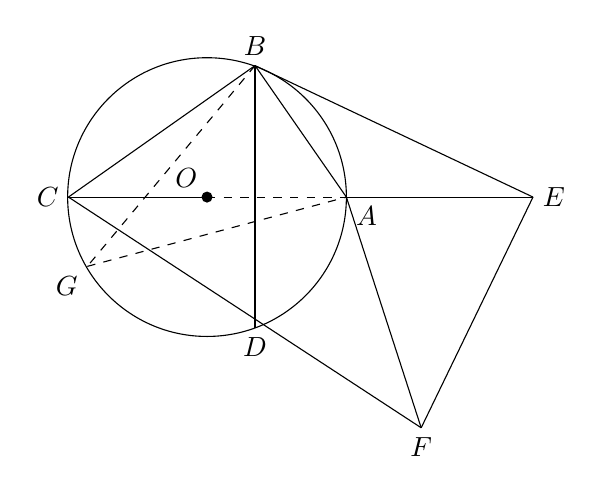
\begin{tikzpicture}[scale=1]
  % 圆 (圆心 O，半径约 1.77)
  \draw (0,0) circle (1.77);
  \fill (0,0) circle (2pt);

  % 圆心 O 的标签
  \node[above left] at (0,0) {$O$};

  % 实线部分：C 到 O，A 到 E（与 OC、EA 共线的段保持实线）
  \draw (-1.76,0) -- (0,0);
  \draw (1.77,0) -- (4.14,0);

  % 修改部分：线段 AO 改为虚线
  \draw[dashed] (0,0) -- (1.77,0);

  % 其余实线
  \draw (-1.76,0) -- (0.61,1.67);   % CB
  \draw (0.61,1.67) -- (1.77,0);    % BA
  \draw (0.61,1.67) -- (4.14,0);    % BE
  \draw (0.61,1.67) -- (0.61,-1.66);% BD
  \draw (-1.76,0) -- (2.72,-2.93);  % CF
  \draw (1.77,0) -- (2.72,-2.93);   % AF
  \draw (4.14,0) -- (2.72,-2.93);   % EF

  % 虚线部分：BG 与 GA
  \draw[dashed] (0.61,1.67) -- (-1.52,-0.88);  % BG
  \draw[dashed] (-1.52,-0.88) -- (1.77,0);     % GA

  % 顶点标签
  \node[above] at (0.61,1.67) {$B$};
  \node[left] at (-1.76,0) {$C$};
  \node[below right] at (1.77,0) {$A$};
  \node[right] at (4.14,0) {$E$};
  \node[below] at (0.61,-1.66) {$D$};
  \node[below left] at (-1.52,-0.88) {$G$};
  \node[below] at (2.72,-2.93) {$F$};
\end{tikzpicture}
\end{document}
